\chapter{Analýza zadania}

V~tejto kapitole sa zamyslíme nad tým, ako splniť požiadavky definované v~Úvode~(\ref{poziadavky}).

Pre~splnenie požiadavky P1 dáva veľmi dobrý zmysel vytvoriť naše riešenie ako webovú aplikáciu. Týmto spôsobom sa nemusíme starať o~distribúciu programu k~užívateľom. Stačí ak má zákazník~(resp. admin) pripojenie na~internet.

Je síce pravda, že voľba webovej aplikácie zahŕňa i~voľbu hostingu. A~ten nemusí byť lacný. To by mohlo byť v~rozpore s~P2. Ale je potrebné dodať, že ak by sme zvolili klasickú desktopovú aplikáciu, tak by sme ju museli nejakým spôsobom dodať zákazníkovi. A~to by bolo nepraktické, prípadne by mohlo stáť takisto nejaké peniaze. Navyše práve webová aplikácia má~potenciál pomôcť firme tak, že ju zákazník objaví pri surfovaní internetu.

Pre splnenie~P4,~P5~a~P8 je jasné, že budeme potrebovať databázu. A~to na~to, aby si firmy vedeli samé tvoriť ponuku, ktorú si do databázy uložia. Po~príchode zákazníka bude možné ponuku z~databázy načítať a~zobraziť. Podobne v~prípade~P8. Keď sa užívateľ zaregistruje, jeho údaje sa uložia v~databáze a~pri prihlásení sa z~nej prečítajú a~môžu použiť pre vyplnenie formulárov podľa potreby.

Znova sa vrátim k~P5. Kedže ide o aukciu, budeme potrebovať nejaký mechanizmus, ktorý by vedel zabezpečiť odpočet, a~takisto vyhodnotenie aukcie na~pozadí. Taktiež si musíme rozmyslieť, ako sa má aukcia správať v~rôznych situáciách.

Na to, aby sme splnili P6, musí byť náš softvér schopný posielať správy. Z~podmienky P3 usudzujeme, že nikto nebude pri softvére sedieť, a~teda posielanie dopytov by nemalo mať povahu četu. Posielanie správ bude prebiehať prostredníctvom emailov. To nám vytvára novú požiadavku na~softvér. Aby administrátor nemusel preklikávať medzi svojou emailovou schránku a~naším systémom, bolo by dobre integrovať jeho schránku priamo do systému.

\section{Voľba typu aplikácie, jazyka a frameworku}

Po prejdení požiadaviek vieme, že chceme vytvoriť webovú aplikáciu s~bohatým uživateľským rozhraním, ktorá by bola schopná posielať a~prijímať správy, pracovať s~databázou, umožnila nám autentikáciu a~autorizáciu, a~taktiež vykonávať prácu na~pozadí. Pre túto úlohu sa hodia vysokoúrovňové jazyky, ako sú napríklad C\# alebo Java\dots Na~základe autorových skúseností si volíme jazyk C\# a platformu .NET, ktorá je s~ním spojená.

Platforma .NET nám pre vývoj webových aplikácií poskytuje framework\\ASP.NET alebo Blazor. Obe frameworky sú si podobné. Rozdiel náj\-de\-me v~tom, že Blazor umožňuje vytváranie komponent. Komponent si môžeme predstaviť ako logickú časť stránky (napr. tabuľka, tlačidlo\dots). Po~zadefinovaní komponentu ho~vieme „recyklovať“. Tým myslím to, že ho môžeme použiť na viacerých miestach na webe. Na~každom mieste sa bude správať a~vyzerať rovnako (príp.~vie\-me  jeho správanie meniť pomocou parametrov). Táto myšlienka komponentov sa autorovi páči, dobre sa s~ňou pracuje a~neskôr si ukážeme ako nám pomôže vyriešiť problém s odpočtom.

Blazor poskytuje viacero hosting modelov. V~čase rozhodovania existovali dva: Blazor WebAssembly a Blazor Server. Výber WebAssembly by zahŕňal niekoľko problémov. Pri~prvotnej návšteve stránky sa musia klientovi stiahnuť zdrojové kódy aplikácie. To môže chvíľu trvať a~mohlo by to odradiť nových potenciálnych zákazníkov. V~prípade Blazor Server tento problém nemáme, pretože kód beží na~serveri a~užívateľovi sa servíruje už len prerenderovaný HTML, CSS, JavaScript kód stránky. Z~rovnakého dôvodu sú weby vytvorené Blazor Ser\-ve\-rom SEO-friendly (čo znamená, že sú dohľadateľné vyhľadávačmi, akým je napríklad~Google). V~prípade WebAssembly môžu mať vyhľadávače problém. Na to, aby sa dostali k obsahu stránky si musia obsah vygenerovať zo stiahnutých zdrojových kódov. Ale  to môžu mať zakázané z~bezpečnostných dôvodov alebo toho nemusia byť schopné. V~súčasnosti webové prehliadače (Google Chrome, Mozilla Firefox, \dots) podporujú WebAssembly. Ale autor pozorovaním zistil, že vo~firmách sa zvyknú využívať staré počítače s~potenciálne starým softvérom. Takže hrozí, že by sme mali problém WebAssembly rozbehnúť. Kvôli spomenutým dôvodom si volíme Blazor Server.

\section{Návrh systému}

V Úvode sme rozhodli, že náš systém je webová aplikácia, ktorá pracuje s~databázou. Webová aplikácia funguje ako rozhranie pre interakciu s~užívateľmi. Databázu potrebujeme kvôli perzistencii dát. Ako vidíme, obe časti poskytujú vlastnú funkcionalitu. Ak tieto časti oddelíme, pomôžeme rozšíriteľnosti systému.

Keď už vidíme, že systém je zložený z~dvoch častí, poďme si rozmysllieť ako budú spolu interagovať. Webová aplikácia potrebuje pre svoje fungovanie dáta. Tejto závislosti sa nezbavíme. Lenže dátova časť nepotrebuje webovú aplikáciu pre svoje fungovanie. Závislosť z~tejto strany neexistuje.

Majme preto dva projekty: ServISData a ServISWebApp. ServISData slúži ako dátová časť, ktorá je nezávislá a~ServISWebApp poslúži ako webová aplikácia, ktorá je závislá na dátach z projektu ServISData. Architektúru demonštruje obrázok~\ref{architektura systemu}.

\begin{figure}[H]\centering
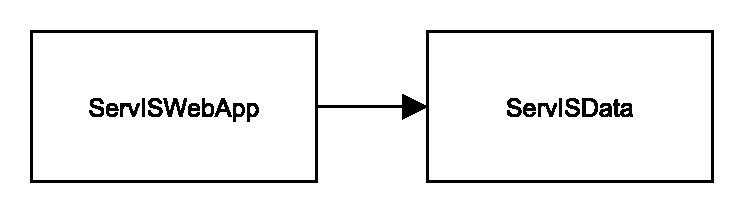
\includegraphics[width=140mm]{../img/architektura systemu}
\caption{Architektúra systému (predstavuje závislosť ServISWebApp od ServISData).}
\label{architektura systemu}
\end{figure}

\section{Voľba databázy}

Vieme, že náš systém potrebuje pre splnenie podmienok~P4, P5 a~P8 databázu. V tejto kapitole si vyberieme typ databázy, databazový server a~rozoberieme si aké entity potrebujeme.

\subsection{Návrh relačného modelu databázy}

Z P4 vieme, že potrebujeme entity pre bagre a~prídavné zariadenia. Niekoho by mohlo napadnúť spojiť obe entity do~jednej, ale to my nespravíme. Ide o~rozdielne entity, ktoré môžu uchovávať rozdielne informácie (a~ako neskôr v~texte uvidíme, skutočne budú uchovávať rozdielne dáta).

Kedže ide o~ponuku, ktorú chceme prezentovať zákazníkom, chceme okrem textových údajov prezentovať položku, či už stroj alebo~prídavné zariadenie, pomocou fotky. A~nie jednej (predpokladám, že položku budú chcieť firmy predviesť zákazníkom z viacerých uhlov). Znovu by niekomu mohlo napadnúť, že by bol dobrý nápad zlúčiť entitu fotky stroja s~entitou fotky prídavného zariadenia. Ale tieto veci nie sú totožné. Ak by sme entity zlúčili (a~mali teda iba 1 entitu pre~fotku všeobecne), tak by existovala možnosť priradiť fotku prídaného zariadenia stroju (a~naopak). Ale to je nesprávne. Preto znova vytvoríme dve entity. Jedna bude fotka stroja, druhá bude fotka prídavného zariadenia. Pre fotku stroja platí, že patrí práve jednému stroju. Stroj môže mať viacero fotiek. Analogicky platí pre prídavné zariadenia a~ich fotky.

Pri strojoch sa ešte zastavíme. Existujú rôzne značky strojov (napr. Locust, Eurocomach,\dots), a takisto rôzne ketegórie strojov (napr. šmykom riadené nakladače, pásové bagre,\dots). Ďalej v texte, keď budem používať spojenie typ stroja, tak tým myslím kombináciu značky stroja a kategórie stroja. Každý typ stroja sa môže líšiť druhom a formou údajov. Napríklad typ A má hmotnosť ako vlastnosť, ktorú chceme spolu so zbytkom údajov zobraziť užívateľovi. Ďalej typ B má namiesto hmotnosti údaj o výške stroja. Existujú údaje (ako sú napr. meno a opis stroja), ktoré existujú pre každý stroj. Ale takisto existujú údaje, ktoré sa líšia v závislosti od typu stroja. Takýmito údajmi sú vlastnosti stroja. Ako budeme tieto premenlivé údaje ukladať? Jedno z riešení, ktoré by nás mohlo napadnúť je vytvoriť rodičovskú entitu, ktorá by obsahovala údaje spoločné pre všetky typy strojov. A v entitách, ktoré by dedili od rodičovskej triedy by sme dodefinovali premenlivé vlastnosti. Toto riešenie by pravdepodobne fungovalo, lenže má zásadnú nevýhodu. Zakaždým keď si firma zmyslí, že potrebuje nový typ stroja, by entita musela byť manuálne doprogramovaná. Ale kedže my chceme systém navrhnúť všeobecne tak, aby si každá firma vedela zadefinovať vlastnú ponuku strojov, volíme inú alternatívu. Vytvoríme si entitu pre typ stroja. Každý stroj bude nejakého typu. Každý typ obsahuje údaj o~značke a~kategórii. Značka a~kategória sú tiež ďalšími entitami. Typ stroja určuje, akého typu budú vlastnosti konkrétneho stroja. Takže budeme potrebovať entitu typ vlastnosti stoja. Tá obsahuje údaje: názov vlastnosti (napr. hmotnosť, výška,\dots) a~typ hodnoty vlastnosti (napr. číslo, text,\dots). Teda admin bude môcť priradiť typu stroja akého typu bude mať konkrétny stroj vlastnosti.

Stroj vie svoj typ, a~ten vie aké (akého typu) má konkrétny stroj vlastnosti. To, čo ešte nevieme, sú konkrétne hodnoty vlastností stroja. Dovolím si vysvetliť na~príklade. Momentálne máme informáciu o~tom, že konkrétny stroj~S, typu~T, má vlasnosť hmotnosť, ale stále nevieme konkrétnu hodnotu, teda stále nevieme koľko váži. Preto vytvoríme entitu reprezentujúcu vlastnosť stroja. Táto entita vie, akého je typu. A~takisto v~sebe uchováva konkrétnu hodnotu vlastnosti (v~kontexte príkladu, uchováva v~sebe váhu stroja). Každý stroj má v~sebe toľko vlastností, koľko ich je zadefinovaných v~jeho type.

Teraz sa vráťme k~prídavným zariadeniam. Každé prídavné zariadenie má, podobne ako stroj, takisto svoju značku a~patrí do nejakej kategórie. Navyše má oproti strojom aj údaj o~tom, pre akú kategóriu strojov je zariadenie vytvorené. Avšak na rozdiel od~predošlého prípadu so~strojmi, sa tento prípad líši v~tom, že každé prídavné zariadenie, bez ohľadu na~kombináciu typu, kategórie a~kategórie stroja, má druh a~formu údajov rovnakú. Takže stačí ak vytvoríme entitu pre~značku a~kategóriu prídavného zariadenia (entitu pre kategóriu stroja už máme) a~entita reprezentujúca prídavné zariadenie si bude v~sebe držať informáciu o~tom, akej je značky, kategórie a~pre akú kategóriu strojov je vytvorená.

Aby sme splnili P5, budeme potrebovať entitu reprezentujúcu aukčnú ponuku. Aukčná ponuka bude držať informáciu o~tom, aký stroj je v~dražbe. A~takisto údaje o~ponuke (napr. vyvolávacia cena, koniec aukcie,\dots).

No okrem udržania údajov o~aukčnej ponuke a~draženom stroji, si musíme zapamätať i~údaje o~ponukách užívateľov, ktorý sa do~aukcie zapojili. Preto si vytvoríme entitu reprezentujúcu ponuku užívateľa. Bude v~sebe niesť údaje o~tom, ktorý úžívateľ ponúkol sumu, v~akej výške a~pre ktorú aukčnú ponuku.

Entitu užívateľa som načal už v~prechádzajúcom odstavci. Túto entitu skutočne budeme potrebovať a~to aj kvôli splneniu P8. Údaje užívateľov musíme pri~registrácii uchovať, aby sme nimi vedeli predvypĺniť formuláre, a~takisto aby sme vedeli vytvoriť prihlasovanie.

Čítateľ by mohol navrhnúť, že pre splnenie P6 budeme potrebovať entitu reprezentujúcu správy. Toto riešenie by mohlo fungovať, ale ako si neskôr ukážeme, existuje aj iné riešenie. Také, ktoré nám ušetrí úložisko v~databáze a navyše uľahčí implementáciu. Preto entitu pre správy nevytvárame.

Pre splnenie P7 si vytvoríme entitu, ktorá bude reprezentovať náhradné diely stroja. Každý náhradný diel bude niesť informáciu o~tom, v~ktorých strojoch sa nachádza. A~každý stroj bude vedieť aké diely obsahuje. Každý náhradný diel obsahuje katalógové číslo. Toto číslo je unikátne medzi strojmi, a~preto by mohlo byť použité ako primárny kľúč entity. Ale autor sa z opatrnosti a~kvôli konzistencii (každá entita má id) rozhodol využiť ako primárny kľúč id i~pri náhradných dieloch.

Hlavným predmetom predaja sú stroje. A~preto chceme aby prvé, čo zákazník po~príchode na~stránku uvidí bola ponuka strojov. Takže ešte budeme potrebovať entitu na~reprezentáciu hlavnej ponuky. Táto entita vie aký typ strojov ponúka, a~zároveň obsahuje reprezentatívnu fotku a~opis strojov daného typu.

Pre detailnejšiu predstavu môžeme návrh vidieť na~obrázku~\ref{relacny model uml}.

\begin{figure}[H]\centering
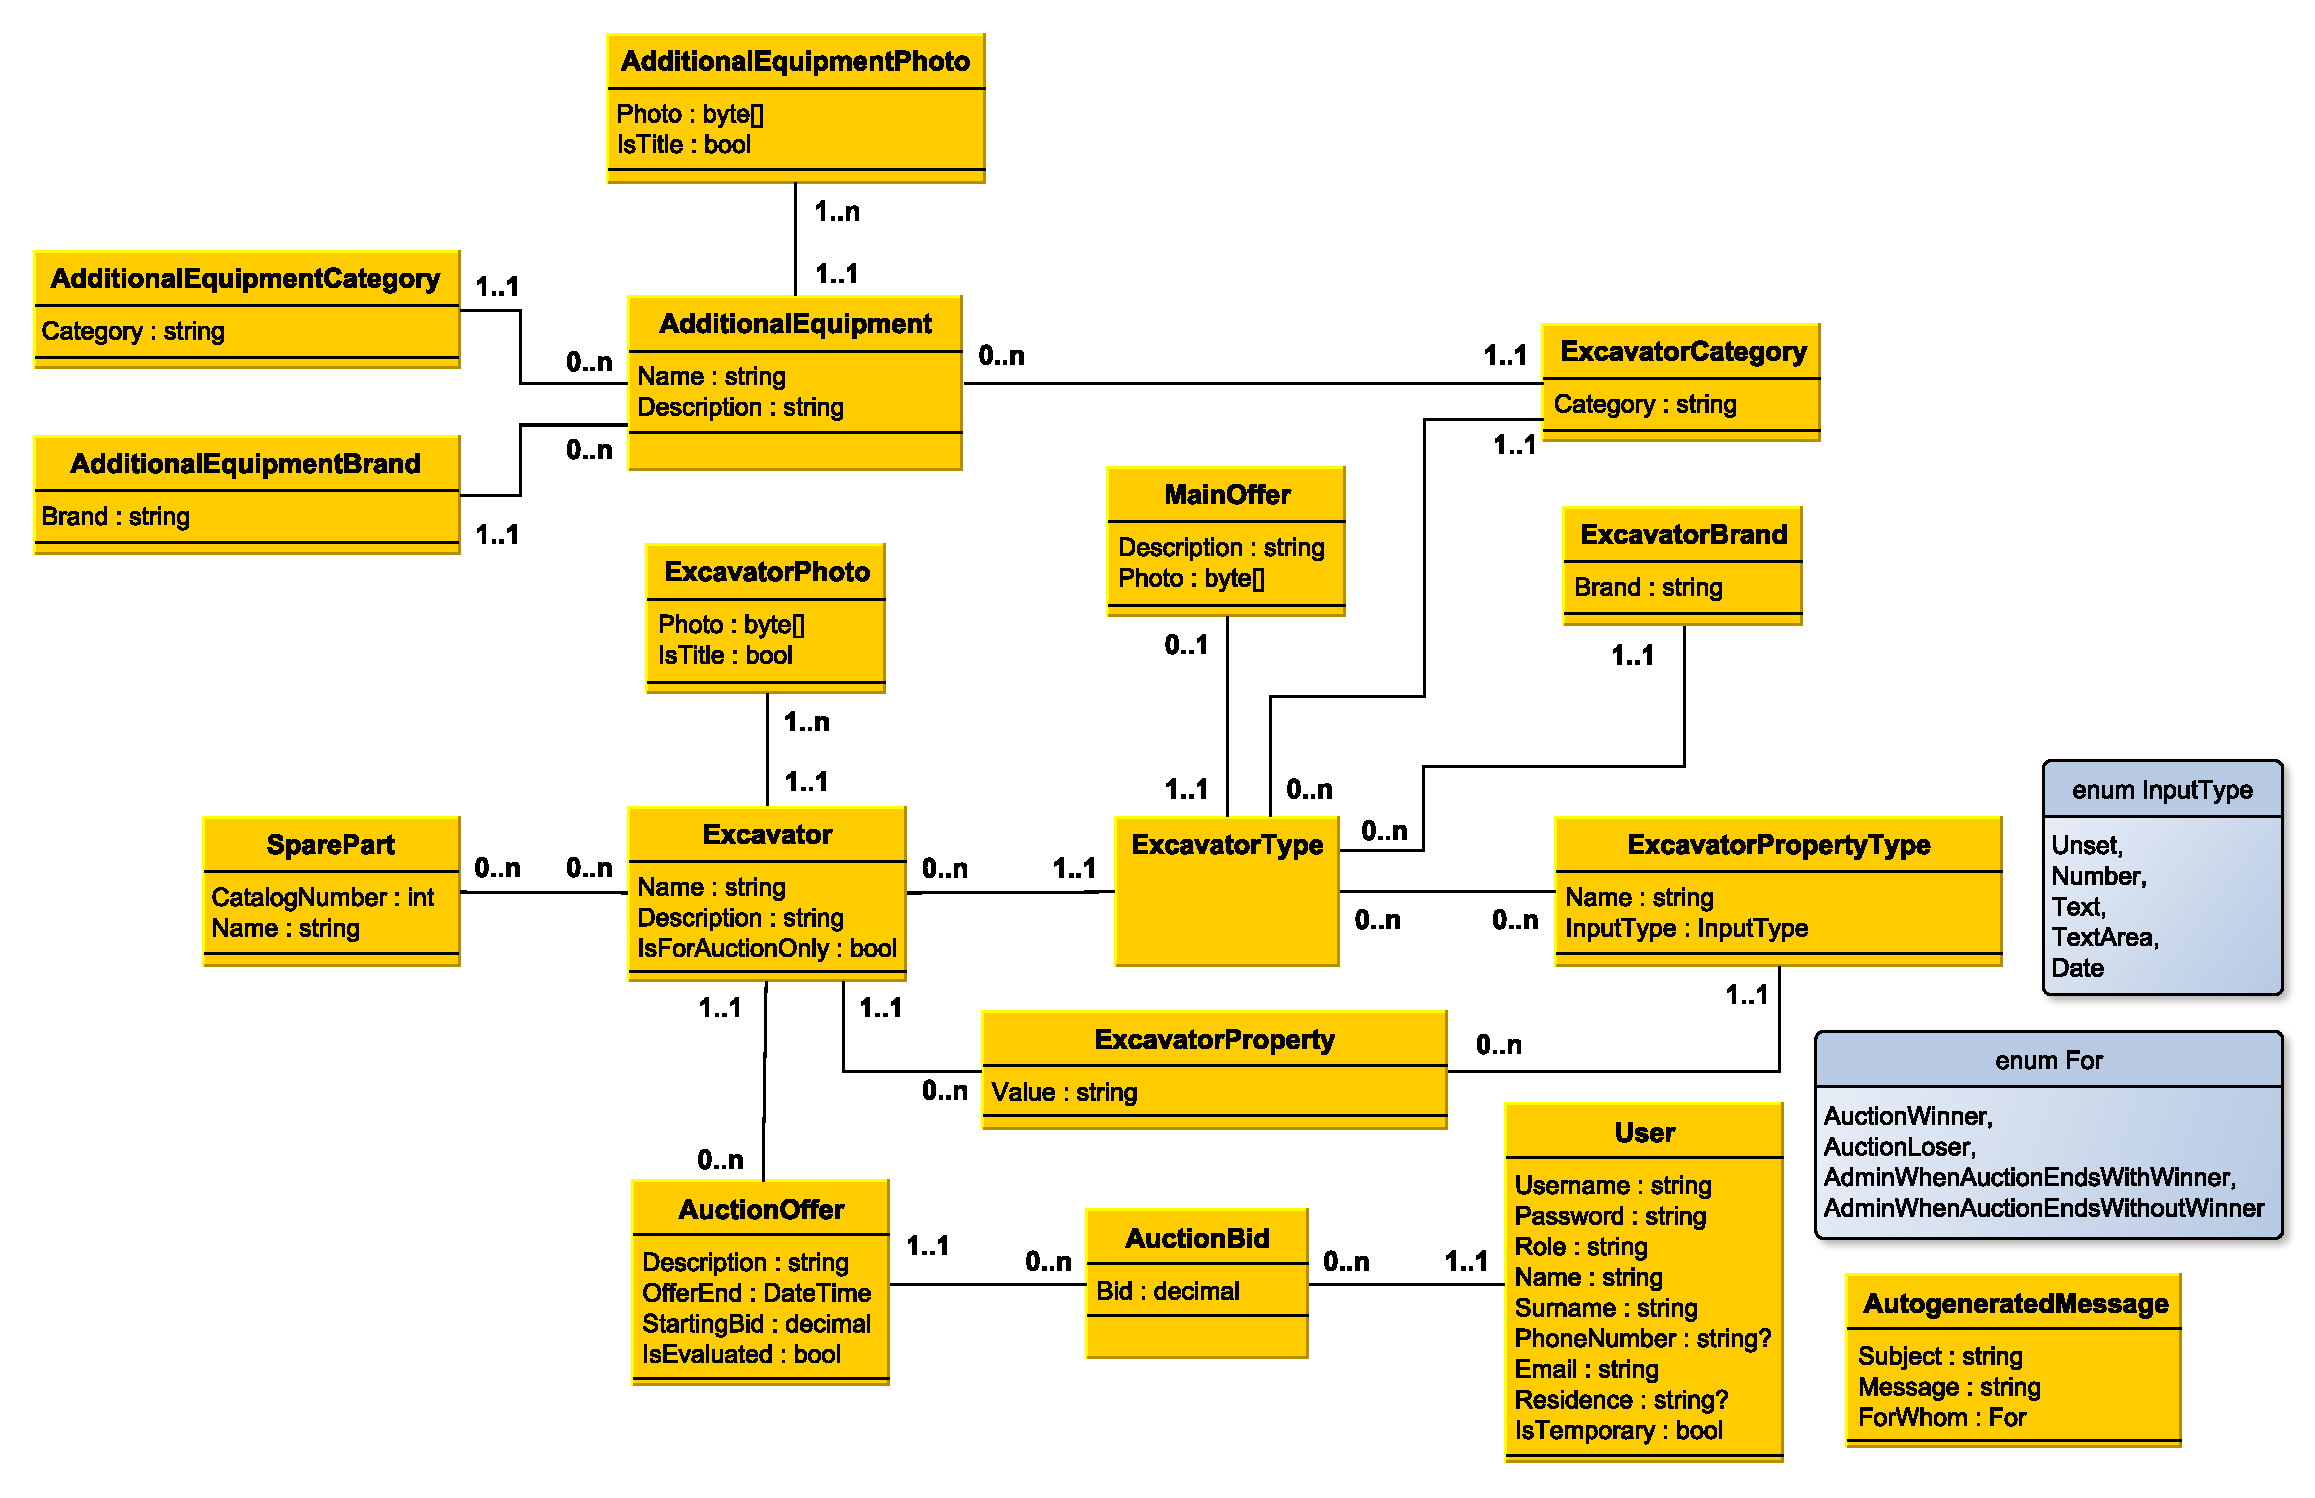
\includegraphics[width=140mm]{../img/relacny model uml}
\caption{Relačný model databázy.}
\label{relacny model uml}
\end{figure}

\subsection{Voľba typu databázy a databázového servera}

TBA

\subsection{ORM}

Prečo by sme chceli ORM.

\section{Aukcia- odpočet a vyhodnocovanie}

V tejto podkapitole predstavím BackgroundServices?, vysvetlím ako odpočítavať (len 1 timer, v osobitnej komponente kvôli rerenderom), ako funguje vyhodnocovanie- rozne scenare (co sa stane ak mame vitaza, co sa stane ak nemamee vitaza).

\section{Posielanie a príjimanie správ}

V tejto podkapitole rozoberieme spôsoby ako posielať/prijímať správy. Gmail api? AE.net? Mailkit?
